\documentclass{article}

\usepackage{lipsum}
\usepackage[margin=1in,includefoot]{geometry}
\usepackage{graphicx}
\usepackage{float}
\usepackage[hidelinks]{hyperref}
\usepackage{amsmath}
\usepackage{amssymb}
\usepackage{color}


\usepackage[usenames,dvipsnames]{xcolor}
\usepackage{listings}







% Header and Footer Stuff
\usepackage{fancyhdr}
\pagestyle{fancy}
\fancyhead{}
\fancyfoot{}
\fancyfoot[R]{\thepage}
\renewcommand{\headrulewidth}{0pt}
\renewcommand{\footrulewidth}{0pt}


\definecolor{dkgreen}{rgb}{0,0.6,0}
\definecolor{gray}{rgb}{0.5,0.5,0.5}
\definecolor{mauve}{rgb}{0.58,0,0.82}

\lstset{
  language=VHDL,
  aboveskip=3mm,
  belowskip=3mm,
  showstringspaces=false,
  columns=flexible,
  basicstyle={\small\ttfamily},
  numbers=none,
  numberstyle=\tiny\color{gray},
  keywordstyle=\color{blue},
  commentstyle=\color{dkgreen},
  stringstyle=\color{mauve},
  breaklines=true,
  breakatwhitespace=true,
  tabsize=3
}












\begin{document}

\begin{titlepage}
	\begin{center}
	\begin{align*}
	
\includegraphics[height=1.75in]{logo.png}
	\end{align*}


	
	\line(1,0){300}\\
	[0.25in]
	\huge{\bfseries Datapath Design}\\
	[2mm]
	\line(1,0){200}\\
	[1.5cm]
	\textsc{\LARGE Laboratory 2}\\
	[0.75cm]
	\textsc{\Large CS2022 Computer Architecture}\\
	[7cm]	
	\end{center}
	
	
	
	\begin{flushright}
	\textsc{\large Alexandru Sulea\\
	D Stream\\
	\#12315152\\
	11 March 2016\\}
	\end{flushright}
	
	
	
	

\end{titlepage}
%Table of Contents Stuff%
\tableofcontents
%\listoffigures
%\addcontentsline{toc}{section}{List of Figures}
\listoftables
\addcontentsline{toc}{section}{List of Tables}


\thispagestyle{empty}
\cleardoublepage
\pagenumbering{arabic}
\setcounter{page}{1}

\pagebreak
\section{CODE}

\subsection{DATA PATH}\label{sec:intro}

\begin{lstlisting}
library IEEE;
use IEEE.STD_LOGIC_1164.ALL;

entity datapath is
Port ( data_in : in  STD_LOGIC_VECTOR(15 downto 0);
				constant_in : in  STD_LOGIC_VECTOR(15 downto 0);
           D_select : in  STD_LOGIC_VECTOR(16 downto 0);
			  D_Clk : in STD_LOGIC;
           D_Vout : out  STD_LOGIC;
			  D_Cout : out  STD_LOGIC;
			  D_Nout : out  STD_LOGIC;
			  D_Zout : out  STD_LOGIC;
			  address_out : out  STD_LOGIC_VECTOR(15 downto 0);
           data_out : out  STD_LOGIC_VECTOR(15 downto 0));

end datapath;

architecture Behavioral of datapath is
component  mux3_16bit
    Port ( s : in  STD_LOGIC;
           In0 : in  STD_LOGIC_VECTOR(15 downto 0);
           In1 : in  STD_LOGIC_VECTOR(15 downto 0);
           Z : out  STD_LOGIC_VECTOR(15 downto 0));
end Component;

Component function_unit
Port ( F_A : in  STD_LOGIC_VECTOR(15 downto 0);
           F_B : in  STD_LOGIC_VECTOR(15 downto 0);
           F_select : in  STD_LOGIC_VECTOR(4 downto 0);
           F_Vout : out  STD_LOGIC;
			  F_Cout : out  STD_LOGIC;
			  F_Nout : out  STD_LOGIC;
			  F_Zout : out  STD_LOGIC;
           F_F : out  STD_LOGIC_VECTOR(15 downto 0));
end Component;

Component register_file 
    Port ( inA : in  STD_LOGIC_VECTOR(2 downto 0);
           inB : in  STD_LOGIC_VECTOR(2 downto 0);
           inD : in  STD_LOGIC_VECTOR(2 downto 0);
           Clk : in  STD_LOGIC;
          load_in : in  STD_LOGIC;
           data : in  STD_LOGIC_VECTOR(15 downto 0);
				outA :  out  STD_LOGIC_VECTOR(15 downto 0);
				outB :  out  STD_LOGIC_VECTOR(15 downto 0));
end Component ;

signal src_muxD, src_muxB, src_regA, src_regB, src_out : STD_LOGIC_VECTOR(15 downto 0);

begin
Dreg_mux3_16bit : mux3_16bit PORT MAP ( s => D_select(1),
           In0 => src_out,
           In1 => data_in,
           Z => src_muxD);

Breg_mux3_16bit : mux3_16bit PORT MAP ( s => D_select(7),
           In0 => constant_in,
           In1 => src_regB,
           Z => src_muxB);

reg_function_unit: function_unit PORT MAP ( F_A => src_regA,
           F_B => src_muxB,
           F_select => D_select(6 downto 2),
           F_Vout => D_Vout,
			  F_Cout => D_Cout,
			  F_Nout => D_Nout,
			  F_Zout => D_Zout,
           F_F => src_out);

reg_register_file : register_file PORT MAP( inA => D_select(13 downto 11),
           inB => D_select(10 downto 8),
           inD => D_select(16 downto 14),
           Clk => D_Clk,
          load_in => D_select(0),
           data => src_muxD,
				outA => src_regA,
				outB => src_regB);
				
data_out <= src_muxB;
address_out <= src_regA;
end Behavioral;
\end{lstlisting}

\begin{align*}
\centering
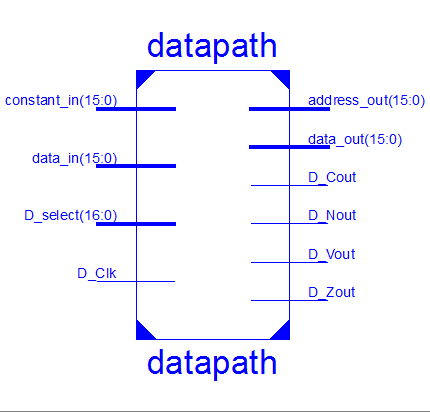
\includegraphics[height=1.5in]{data.png}
\break
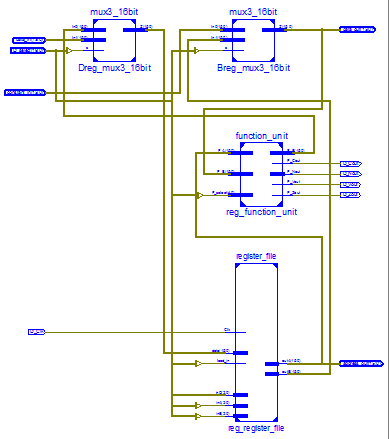
\includegraphics[height=3in]{data2.png}
\end{align*}\\
\pagebreak


\subsection{REGISTER FILE}\label{sec:intro}

\begin{lstlisting}

library IEEE;
use IEEE.STD_LOGIC_1164.ALL;
use IEEE.STD_LOGIC_ARITH.ALL;
use IEEE.STD_LOGIC_UNSIGNED.ALL;


entity register_file is
    Port ( 
           inA : in  STD_LOGIC_VECTOR(2 downto 0);
           inB : in  STD_LOGIC_VECTOR(2 downto 0);
           inD : in  STD_LOGIC_VECTOR(2 downto 0);
           Clk : in  STD_LOGIC;
          load_in : in  STD_LOGIC;
           data : in  STD_LOGIC_VECTOR(15 downto 0);
				outA :  out  STD_LOGIC_VECTOR(15 downto 0);
				outB :  out  STD_LOGIC_VECTOR(15 downto 0)
			 );
end register_file;

architecture Behavioral of register_file is

	Component decoder_3to8
	Port ( A0 : in  STD_LOGIC;
          A1 : in  STD_LOGIC;
			 A2 : in  STD_LOGIC;
          Q0 : out  STD_LOGIC;
          Q1 : out  STD_LOGIC;
          Q2 : out  STD_LOGIC;
          Q3 : out  STD_LOGIC;
          Q4 : out  STD_LOGIC;
          Q5 : out  STD_LOGIC;
          Q6 : out  STD_LOGIC;
          Q7 : out  STD_LOGIC);
	End Component;

	Component mux3_16bit
	Port ( s : in  STD_LOGIC;
          In0 : in  STD_LOGIC_VECTOR(15 downto 0);
          In1 : in  STD_LOGIC_VECTOR(15 downto 0);
          Z : out  STD_LOGIC_VECTOR(15 downto 0));
	End Component;
	
	Component reg8
	Port ( load0 : in  STD_LOGIC;
				load1 : in STD_LOGIC;
          Clk : in  STD_LOGIC;
          D : in  STD_LOGIC_VECTOR(15 downto 0);
          Q : out  STD_LOGIC_VECTOR(15 downto 0));
	End Component;
	
	Component mux8_16bit
	Port ( S0 : in  STD_LOGIC;
           S1 : in  STD_LOGIC;
           S2 : in  STD_LOGIC;
           In0 : in  STD_LOGIC_VECTOR(15 downto 0);
           In1 : in  STD_LOGIC_VECTOR(15 downto 0);
           In2 : in  STD_LOGIC_VECTOR(15 downto 0);
           In3 : in  STD_LOGIC_VECTOR(15 downto 0);
           In4 : in  STD_LOGIC_VECTOR(15 downto 0);
           In5 : in  STD_LOGIC_VECTOR(15 downto 0);
           In6 : in  STD_LOGIC_VECTOR(15 downto 0);
           In7 : in  STD_LOGIC_VECTOR(15 downto 0);
           Z : out  STD_LOGIC_VECTOR(15 downto 0));
	End Component;
	
	signal load_reg0, load_reg1, load_reg2, load_reg3, load_reg4,
				load_reg5, load_reg6, load_reg7 : STD_LOGIC;
	signal reg0_q, reg1_q, reg2_q, reg3_q, reg4_q, reg5_q, reg6_q,
				reg7_q, d_mux, src_reg, src_A, src_B : STD_LOGIC_VECTOR(15 downto 0);

begin
	reg_decoder_3to8 : decoder_3to8 PORT MAP(
		A0 => inD(0),
		A1 => inD(1),
		A2 => inD(2),
		Q0 => load_reg0,
		Q1 => load_reg1,
		Q2 => load_reg2,
		Q3 => load_reg3,
		Q4 => load_reg4,
		Q5 => load_reg5,
		Q6 => load_reg6,
		Q7 => load_reg7
		);
	
	A_reg_mux8_16bit : mux8_16bit PORT MAP(
		S0 => inA(0),
		S1 => inA(1),
		S2 => inA(2),
		In0 => reg0_q,
		In1 => reg1_q,
		In2 => reg2_q,
		In3 => reg3_q,
		In4 => reg4_q,
		In5 => reg5_q,
		In6 => reg6_q,
		In7 => reg7_q,
		Z => src_A
		);
		
	B_reg_mux8_16bit : mux8_16bit PORT MAP(
		S0 => inB(0),
		S1 => inB(1),
		S2 => inB(2),
		In0 => reg0_q,
		In1 => reg1_q,
		In2 => reg2_q,
		In3 => reg3_q,
		In4 => reg4_q,
		In5 => reg5_q,
		In6 => reg6_q,
		In7 => reg7_q,
		Z => src_B
		);
		
	reg00 : reg8 PORT MAP(
		load0 =>	load_reg0,
		load1 => load_in,
		Clk =>	Clk,
		D =>	data,
		Q => reg0_q);
		
	reg01 : reg8 PORT MAP(
		load0 =>	load_reg1,
		load1 => load_in,
		Clk =>	Clk,
		D =>	data,
		Q => reg1_q);
	
	reg02 : reg8 PORT MAP(
		load0 =>	load_reg2,
		load1 => load_in,
		Clk =>	Clk,
		D =>	data,
		Q => reg2_q);	

	reg03 : reg8 PORT MAP(
		load0 =>	load_reg3,
		load1 => load_in,
		Clk =>	Clk,
		D =>	data,
		Q => reg3_q);

	reg04 : reg8 PORT MAP(
		load0 =>	load_reg4,
		load1 => load_in,
		Clk =>	Clk,
		D =>	data,
		Q => reg4_q);
		
	reg05 : reg8 PORT MAP(
		load0 =>	load_reg5,
		load1 => load_in,
		Clk =>	Clk,
		D =>	data,
		Q => reg5_q);
		
	reg06 : reg8 PORT MAP(
		load0 =>	load_reg6,
		load1 => load_in,
		Clk =>	Clk,
		D =>	data,
		Q => reg6_q);
		
	reg07 : reg8 PORT MAP(
		load0 =>	load_reg7,
		load1 => load_in,
		Clk =>	Clk,
		D =>	data,
		Q => reg7_q);

	outA <= src_A;
	outB <= src_B;


end Behavioral;

\end{lstlisting}



\begin{align*}
\centering
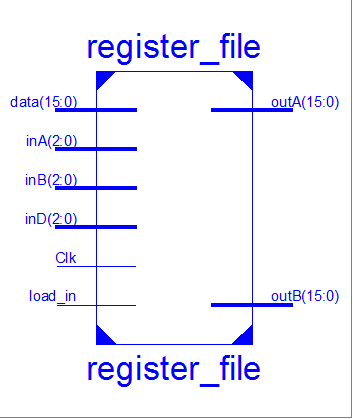
\includegraphics[height=1.5in]{register1.png}
\break
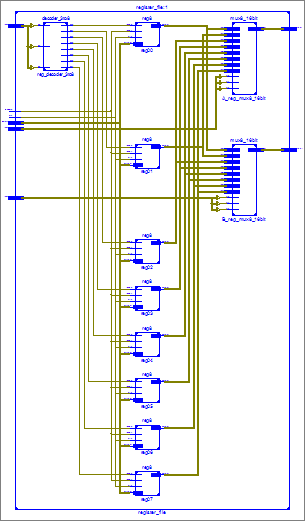
\includegraphics[height=3in]{register2.png}
\end{align*}\\



\pagebreak
\subsubsection{REG8}\label{sec:result}

\begin{lstlisting}
library IEEE;
use IEEE.STD_LOGIC_1164.ALL;
use IEEE.STD_LOGIC_ARITH.ALL;
use IEEE.STD_LOGIC_UNSIGNED.ALL;
entity reg8 is
    Port ( load0 : in  STD_LOGIC;
			  load1 : in  STD_LOGIC;
           Clk : in  STD_LOGIC;
           D : in  STD_LOGIC_VECTOR(15 downto 0);
           Q : out  STD_LOGIC_VECTOR(15 downto 0));
end reg8;

architecture Behavioral of reg8 is

begin
process(Clk)
begin 
		if(rising_edge(Clk)) then 
			if(load0 ='1') and (load1 ='1') then 
				Q<= D after 5ns;
			end if;
		end if;
	end process;
end Behavioral;
\end{lstlisting}

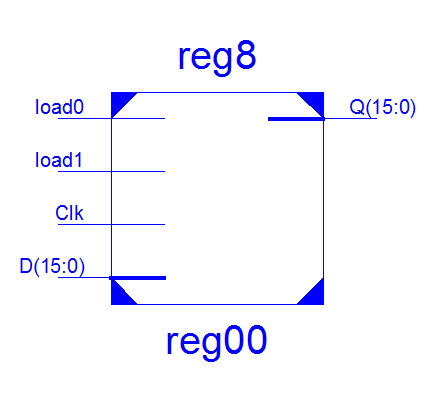
\includegraphics[width=6cm, height=8cm]{reg8.png}


\pagebreak
\subsubsection{DECODER}\label{sec:result}

\begin{lstlisting}
 library IEEE;
use IEEE.STD_LOGIC_1164.ALL;
use IEEE.STD_LOGIC_ARITH.ALL;
use IEEE.STD_LOGIC_UNSIGNED.ALL;


entity decoder_3to8 is
    Port ( A0 : in  STD_LOGIC;
           A1 : in  STD_LOGIC;
           A2 : in  STD_LOGIC;
           Q0 : out  STD_LOGIC;
           Q1 : out  STD_LOGIC;
           Q2 : out  STD_LOGIC;
           Q3 : out  STD_LOGIC;
           Q4 : out  STD_LOGIC;
           Q5 : out  STD_LOGIC;
           Q6 : out  STD_LOGIC;
           Q7 : out  STD_LOGIC);
end decoder_3to8;

architecture Behavioral of decoder_3to8 is

begin
	Q0 <= ((	NOT A0) AND (NOT A1) AND (NOT A2)) AFTER 5ns;
	Q1 <= ((	NOT A0) AND (NOT A1) AND A2) AFTER 5ns;
	Q2 <= ((	NOT A0) AND A1 AND (NOT A2)) AFTER 5ns;
	Q3 <= ((	NOT A0) AND A1 AND A2) AFTER 5ns;
	Q4 <= (A0 AND (NOT A1) AND (NOT A2)) AFTER 5ns;
	Q5 <= (A0 AND (NOT A1) AND A2) AFTER 5ns;
	Q6 <= (A0 AND A1 AND (NOT A2)) AFTER 5ns;
	Q7 <= (A0 AND A1 AND A2) AFTER 5ns;

end Behavioral;
\end{lstlisting}

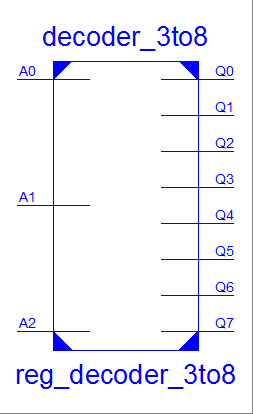
\includegraphics[width=5cm, height=7cm]{decoder.png}
\pagebreak
\subsubsection{MUX3 TO 16BIT}\label{sec:result}

\begin{lstlisting}
library IEEE;
use IEEE.STD_LOGIC_1164.ALL;
use IEEE.STD_LOGIC_ARITH.ALL;
use IEEE.STD_LOGIC_UNSIGNED.ALL;


entity mux3_16bit is
    Port ( s : in  STD_LOGIC;
           In0 : in  STD_LOGIC_VECTOR(15 downto 0);
           In1 : in  STD_LOGIC_VECTOR(15 downto 0);
           Z : out  STD_LOGIC_VECTOR(15 downto 0));
end mux3_16bit;

architecture Behavioral of mux3_16bit is

begin
	Z <= In0 after 5ns when s = '0' else
			In1 after 5ns when s = '1' else
			x"0000" after 5ns;

end Behavioral;

\end{lstlisting}

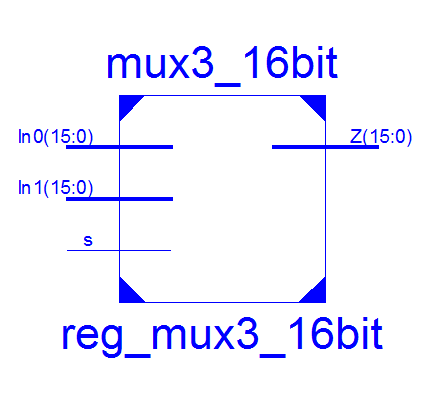
\includegraphics[width=6cm, height=8cm]{mux3to16.png}

\pagebreak
\subsubsection{MUX8 TO 16BIT}\label{sec:result}

\begin{lstlisting}
library IEEE;
use IEEE.STD_LOGIC_1164.ALL;
use IEEE.STD_LOGIC_ARITH.ALL;
use IEEE.STD_LOGIC_UNSIGNED.ALL;


entity mux8_16bit is
    Port ( S0 : in  STD_LOGIC;
           S1 : in  STD_LOGIC;
           S2 : in  STD_LOGIC;
           In0 : in  STD_LOGIC_VECTOR(15 downto 0);
           In1 : in  STD_LOGIC_VECTOR(15 downto 0);
           In2 : in  STD_LOGIC_VECTOR(15 downto 0);
           In3 : in  STD_LOGIC_VECTOR(15 downto 0);
           In4 : in  STD_LOGIC_VECTOR(15 downto 0);
           In5 : in  STD_LOGIC_VECTOR(15 downto 0);
           In6 : in  STD_LOGIC_VECTOR(15 downto 0);
           In7 : in  STD_LOGIC_VECTOR(15 downto 0);
           Z : out  STD_LOGIC_VECTOR(15 downto 0));
end mux8_16bit;

architecture Behavioral of mux8_16bit is

begin
	Z <= In0 after 5ns when S0 = '0' and S1 = '0' and S2 = '0' else 
			In1 after 5ns when S0 = '0' and S1 = '0' and S2 = '1' else 
			In2 after 5ns when S0 = '0' and S1 = '1' and S2 = '0' else 
			In3 after 5ns when S0 = '0' and S1 = '1' and S2 = '1' else
			In4 after 5ns when S0 = '1' and S1 = '0' and S2 = '0' else
			In5 after 5ns when S0 = '1' and S1 = '0' and S2 = '1' else
			In6 after 5ns when S0 = '1' and S1 = '1' and S2 = '0' else
			In7 after 5ns when S0 = '1' and S1 = '1' and S2 = '1' else
			x"0000" after 5ns;
end Behavioral;

\end{lstlisting}

\begin{align*}
\centering
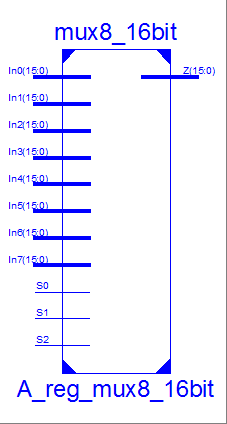
\includegraphics[height=3in]{Amux.png}
\break
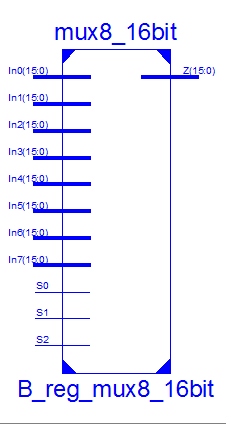
\includegraphics[height=3in]{Bmux.png}
\end{align*}\\

\pagebreak


\subsection{FUNCTION UNIT}\label{sec:result}

\begin{lstlisting}
library IEEE;
use IEEE.STD_LOGIC_1164.ALL;


entity function_unit is
Port ( F_A : in  STD_LOGIC_VECTOR(15 downto 0);
           F_B : in  STD_LOGIC_VECTOR(15 downto 0);
           F_select : in  STD_LOGIC_VECTOR(4 downto 0);
           F_Vout : out  STD_LOGIC;
			  F_Cout : out  STD_LOGIC;
			  F_Nout : out  STD_LOGIC;
			  F_Zout : out  STD_LOGIC;
           F_F : out  STD_LOGIC_VECTOR(15 downto 0));
end function_unit;

architecture Behavioral of function_unit is

Component arithmetic_logic_unit 
    Port ( ALU_A : in  STD_LOGIC_VECTOR(15 downto 0);
           ALU_B : in  STD_LOGIC_VECTOR(15 downto 0);
           ALU_select : in  STD_LOGIC_VECTOR(3 downto 0);
           ALU_Cout : out  STD_LOGIC;
           ALU_Vout : out  STD_LOGIC;
           ALU_G : out  STD_LOGIC_VECTOR(15 downto 0));
end Component;


Component shifter  Port ( B : in  STD_LOGIC_VECTOR(15 downto 0);
           S : in  STD_LOGIC_VECTOR(1 downto 0);
           IR : in  STD_LOGIC;
           IL : in  STD_LOGIC;
           H : out  STD_LOGIC_VECTOR(15 downto 0));
end Component;

Component mux3_16bit Port ( s : in  STD_LOGIC;
           In0 : in  STD_LOGIC_VECTOR(15 downto 0);
           In1 : in  STD_LOGIC_VECTOR(15 downto 0);
           Z : out  STD_LOGIC_VECTOR(15 downto 0));
end Component;

signal src_ALU, src_shift, src_mux : STD_LOGIC_VECTOR(15 downto 0);

begin

reg_arithmetic_logic_unit : arithmetic_logic_unit 
    Port MAP ( ALU_A => F_A,
           ALU_B => F_B,
           ALU_select => F_select(3 downto 0),
           ALU_Cout => F_Cout, 
           ALU_Vout => F_Vout,
           ALU_G => src_ALU);

reg_shifter : shifter  Port MAP ( B => F_B,
           S => F_select(3 downto 2),
           IR => '0',
           IL => '0',
           H => src_shift);


reg_mux3_16bit : mux3_16bit Port MAP ( s => F_select(4),
           In0 => src_ALU,
           In1 => src_shift,
           Z  => src_mux);

F_F <= src_mux;
F_Nout <= src_mux(15);
F_Zout <= ((src_mux(15)) or (src_mux(14)) or (src_mux(13)) or
				(src_mux(12)) or (src_mux(11)) or (src_mux(10)) or 
				(src_mux(9)) or (src_mux(8)) or (src_mux(7)) or 
				(src_mux(6)) or (src_mux(5)) or (src_mux(4)) or 
				(src_mux(3)) or (src_mux(2)) or 
				(src_mux(1)) or (src_mux(0)));



end Behavioral;
\end{lstlisting}


\begin{align*}
\centering
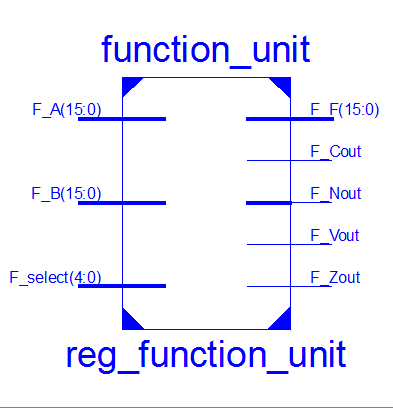
\includegraphics[height=3in]{func1.png}
\break
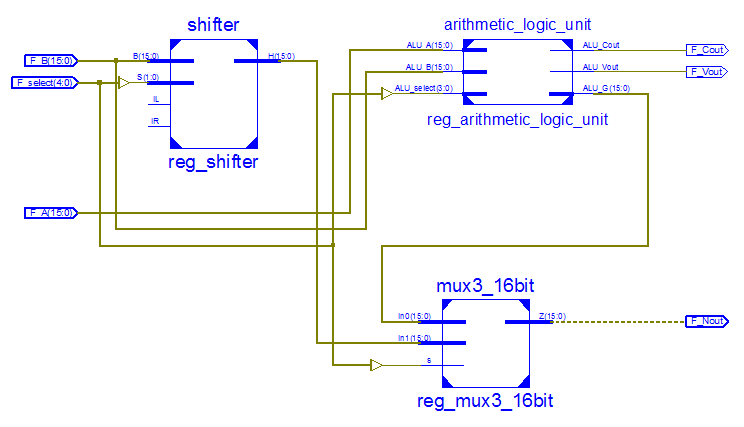
\includegraphics[height=3in]{func2.png}
\end{align*}\\
\pagebreak


\subsection{SHIFTER}\label{sec:result}

\begin{lstlisting}
library IEEE;
use IEEE.STD_LOGIC_1164.ALL;


entity shifter is
    Port ( B : in  STD_LOGIC_VECTOR(15 downto 0);
           S : in  STD_LOGIC_VECTOR(1 downto 0);
           IR : in  STD_LOGIC;
           IL : in  STD_LOGIC;
           H : out  STD_LOGIC_VECTOR(15 downto 0));
end shifter;

architecture Behavioral of shifter is

component  mux3_1bit Port ( In0 : in  STD_LOGIC;
           In1 : in  STD_LOGIC;
           In2 : in  STD_LOGIC;
           S0 : in  STD_LOGIC;
           S1 : in  STD_LOGIC;
           Z : out  STD_LOGIC);
end component;

begin



mux3_1bit00 : mux3_1bit PORT MAP ( In0 =>B(0) ,
           In1 => B(1), 
           In2 => IL,
           S0 => S(0),
           S1 => S(1),
           Z  => H(0));

mux3_1bit01 : mux3_1bit PORT MAP ( In0 =>B(1) ,
           In1 => B(2), 
           In2 => B(0),
           S0 => S(0),
           S1 => S(1),
           Z  => H(1));
			  
mux3_1bit02 : mux3_1bit PORT MAP ( In0 =>B(2) ,
           In1 => B(3), 
           In2 => B(1),
           S0 => S(0),
           S1 => S(1),
           Z  => H(2));

mux3_1bit03 : mux3_1bit PORT MAP ( In0 =>B(3) ,
           In1 => B(4), 
           In2 => B(2),
           S0 => S(0),
           S1 => S(1),
           Z  => H(3));
			  
mux3_1bit04 : mux3_1bit PORT MAP ( In0 =>B(4) ,
           In1 => B(5), 
           In2 => B(3),
           S0 => S(0),
           S1 => S(1),
           Z  => H(4));

mux3_1bit05 : mux3_1bit PORT MAP ( In0 =>B(5) ,
           In1 => B(6), 
           In2 => B(4),
           S0 => S(0),
           S1 => S(1),
           Z  => H(5));
			  
mux3_1bit06 : mux3_1bit PORT MAP ( In0 =>B(6) ,
           In1 => B(7), 
           In2 => B(5),
           S0 => S(0),
           S1 => S(1),
           Z  => H(6));

mux3_1bit07 : mux3_1bit PORT MAP ( In0 =>B(7) ,
           In1 => B(8), 
           In2 => B(6),
           S0 => S(0),
           S1 => S(1),
           Z  => H(7));
			  
mux3_1bit08 : mux3_1bit PORT MAP ( In0 =>B(8) ,
           In1 => B(9), 
           In2 => B(7),
           S0 => S(0),
           S1 => S(1),
           Z  => H(8));

mux3_1bit09 : mux3_1bit PORT MAP ( In0 =>B(9) ,
           In1 => B(10), 
           In2 => B(8),
           S0 => S(0),
           S1 => S(1),
           Z  => H(9));
			  
mux3_1bit10 : mux3_1bit PORT MAP ( In0 =>B(10) ,
           In1 => B(11), 
           In2 => B(9),
           S0 => S(0),
           S1 => S(1),
           Z  => H(10));

mux3_1bit11 : mux3_1bit PORT MAP ( In0 =>B(11) ,
           In1 => B(12), 
           In2 => B(10),
           S0 => S(0),
           S1 => S(1),
           Z  => H(11));
			  
mux3_1bit12 : mux3_1bit PORT MAP ( In0 =>B(12) ,
           In1 => B(13), 
           In2 => B(11),
           S0 => S(0),
           S1 => S(1),
           Z  => H(12));

mux3_1bit13 : mux3_1bit PORT MAP ( In0 =>B(13) ,
           In1 => B(14), 
           In2 => B(12),
           S0 => S(0),
           S1 => S(1),
           Z  => H(13));
			  
mux3_1bit14 : mux3_1bit PORT MAP ( In0 =>B(14) ,
           In1 => B(15), 
           In2 => B(13),
           S0 => S(0),
           S1 => S(1),
           Z  => H(14));

mux3_1bit15 : mux3_1bit PORT MAP ( In0 =>B(15) ,
           In1 => IR, 
           In2 => B(14),
           S0 => S(0),
           S1 => S(1),
           Z  => H(15));
end Behavioral;
\end{lstlisting}

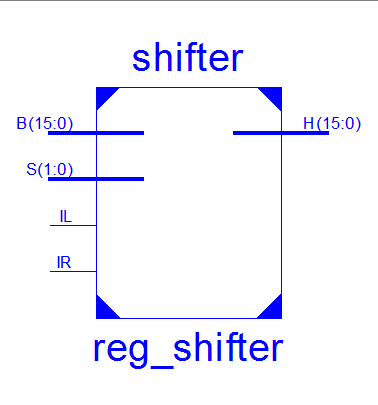
\includegraphics[width=6cm, height=8cm]{shifter.png}
\pagebreak


\subsubsection{MUX3 TO 1BIT}\label{sec:result}

\begin{lstlisting}
library IEEE;
use IEEE.STD_LOGIC_1164.ALL;


entity mux3_1bit is
    Port ( In0 : in  STD_LOGIC;
           In1 : in  STD_LOGIC;
           In2 : in  STD_LOGIC;
           S0 : in  STD_LOGIC;
           S1 : in  STD_LOGIC;
           Z : out  STD_LOGIC);
end mux3_1bit;

architecture Behavioral of mux3_1bit is

begin
Z <= In0 after 1ns when S0 = '0' and S1='0' else
		In1 after 1ns when S0 ='0' and S1= '1' else
		In2 after 1ns when S0 ='0' and S1 = '0' else
		'0' after 1ns;

end Behavioral;
\end{lstlisting}


\pagebreak


\subsection{ALU}\label{sec:result}

\begin{lstlisting}
library IEEE;
use IEEE.STD_LOGIC_1164.ALL;



entity arithmetic_logic_unit is
    Port ( ALU_A : in  STD_LOGIC_VECTOR(15 downto 0);
           ALU_B : in  STD_LOGIC_VECTOR(15 downto 0);
           ALU_select : in  STD_LOGIC_VECTOR(3 downto 0);
           ALU_Cout : out  STD_LOGIC;
           ALU_Vout : out  STD_LOGIC;
           ALU_G : out  STD_LOGIC_VECTOR(15 downto 0));
end arithmetic_logic_unit;

architecture Behavioral of arithmetic_logic_unit is

component ripple_adder Port ( A : in  STD_LOGIC_VECTOR(15 downto 0);
           B : in  STD_LOGIC_VECTOR(15 downto 0);
           Cin : in  STD_LOGIC;
           Cout : out  STD_LOGIC;
           Gout : out  STD_LOGIC_VECTOR(15 downto 0);
           Vout : out  STD_LOGIC);
End Component;

component mux3_16bit Port ( s : in  STD_LOGIC;
           In0 : in  STD_LOGIC_VECTOR(15 downto 0);
           In1 : in  STD_LOGIC_VECTOR(15 downto 0);
           Z : out  STD_LOGIC_VECTOR(15 downto 0));
End Component;

component  B_input_logic Port ( B : in  STD_LOGIC_VECTOR(15 downto 0);
           S : in  STD_LOGIC_VECTOR(1 downto 0);
           Y : out  STD_LOGIC_VECTOR(15 downto 0));
End Component;

Component  logic_circuit Port ( A : in  STD_LOGIC_VECTOR(15 downto 0);
           B : in  STD_LOGIC_VECTOR(15 downto 0);
           Cin : in  STD_LOGIC_VECTOR(1 downto 0);
           Cout : out  STD_LOGIC_VECTOR(15 downto 0));
End Component;

signal src_logic , src_B_input_logic, src_ripple : STD_LOGIC_VECTOR(15 downto 0);

begin


reg_ripple_adder : ripple_adder PORT MAP ( A => ALU_A,
           B => src_logic,
           Cin => ALU_select(0),
           Cout => ALU_Cout,
           Gout => src_ripple,
           Vout => ALU_Vout);


reg_mux3_16bit :mux3_16bit PORT MAP ( s => ALU_select(3),
           In0 => src_ripple,
           In1 => src_B_input_logic,
           Z =>ALU_G);


reg_B_input_logic :  B_input_logic PORT MAP ( B => ALU_B,
           S => ALU_SELECT(2 downto 1),
           Y => src_logic);

reg_logic_circuit : logic_circuit PORT MAP( A => ALU_A ,
           B => ALU_B,
           Cin => ALU_select(2 downto 1),
           Cout => src_B_input_logic);



end Behavioral;
\end{lstlisting}


\begin{align*}
\centering
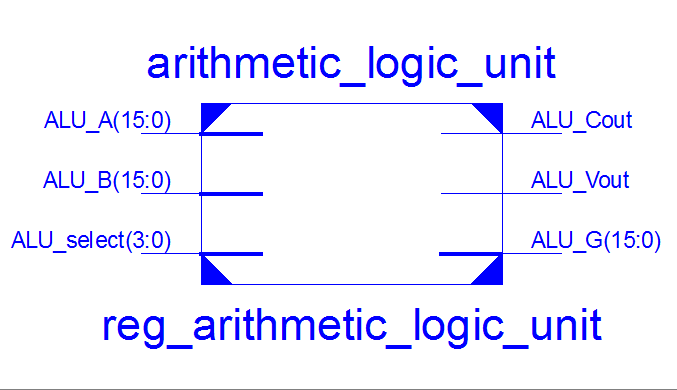
\includegraphics[height=1in]{alu1.png}
\break
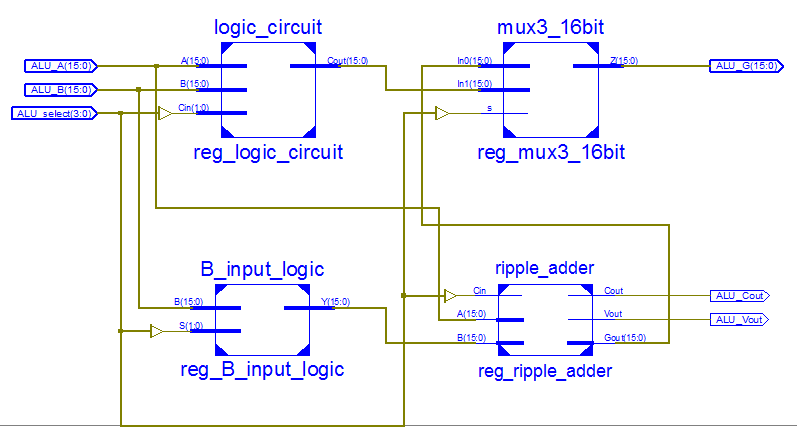
\includegraphics[height=3in]{alu2.png}
\end{align*}\\
\pagebreak



\subsubsection*{LOGIC}\label{sec:result}

\begin{lstlisting}
library IEEE;
use IEEE.STD_LOGIC_1164.ALL;



entity logic_circuit is
    Port ( A : in  STD_LOGIC_VECTOR(15 downto 0);
           B : in  STD_LOGIC_VECTOR(15 downto 0);
           Cin : in  STD_LOGIC_VECTOR(1 downto 0);
           Cout : out  STD_LOGIC_VECTOR(15 downto 0));
end logic_circuit;

architecture Behavioral of logic_circuit is

begin
Cout <= (A and B) after 1ns when Cin = "00" else
			(A or B) after 1ns when Cin = "01" else
			(A xor B) after 1ns when Cin = "10" else
			(not (A)) after 1ns;
end Behavioral;
\end{lstlisting}

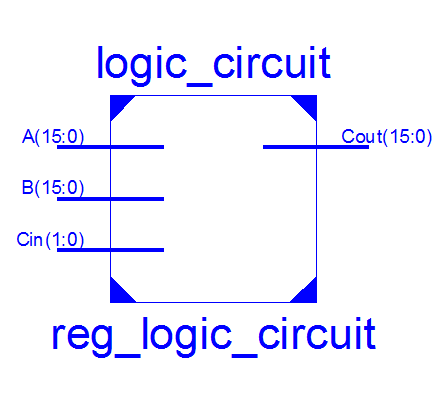
\includegraphics[width=6cm, height=8cm]{logic.png}
\pagebreak



\subsubsection{B LOGIC}\label{sec:result}

\begin{lstlisting}
library IEEE;
use IEEE.STD_LOGIC_1164.ALL;



entity B_input_logic is
    Port ( B : in  STD_LOGIC_VECTOR(15 downto 0);
           S : in  STD_LOGIC_VECTOR(1 downto 0);
           Y : out  STD_LOGIC_VECTOR(15 downto 0));
end B_input_logic;

architecture Behavioral of B_input_logic is

component mux2_1bit  Port ( S0 : in  STD_LOGIC;
										S1 : in  STD_LOGIC;
										Cin : in  STD_LOGIC;
										Res : out  STD_LOGIC);
End Component;

begin
mux2_1bit00 : mux2_1bit PORT MAP( S0 => S(0),
												S1 => S(1),
												Cin =>B(0),
												Res => Y(0));
					
mux2_1bit01 : mux2_1bit PORT MAP( S0 => S(0),
												S1 => S(1),
												Cin =>B(1),
												Res => Y(1));
												
mux2_1bit02 : mux2_1bit PORT MAP( S0 => S(0),
												S1 => S(1),
												Cin =>B(2),
												Res => Y(2));
					
mux2_1bit03 : mux2_1bit PORT MAP( S0 => S(0),
												S1 => S(1),
												Cin =>B(3),
												Res => Y(3));
												
mux2_1bit04 : mux2_1bit PORT MAP( S0 => S(0),
												S1 => S(1),
												Cin =>B(4),
												Res => Y(4));
					
mux2_1bit05 : mux2_1bit PORT MAP( S0 => S(0),
												S1 => S(1),
												Cin =>B(5),
												Res => Y(5));
												
mux2_1bit06 : mux2_1bit PORT MAP( S0 => S(0),
												S1 => S(1),
												Cin =>B(6),
												Res => Y(6));
					
mux2_1bit07 : mux2_1bit PORT MAP( S0 => S(0),
												S1 => S(1),
												Cin =>B(7),
												Res => Y(7));
												
mux2_1bit08 : mux2_1bit PORT MAP( S0 => S(0),
												S1 => S(1),
												Cin =>B(8),
												Res => Y(8));
					
mux2_1bit09 : mux2_1bit PORT MAP( S0 => S(0),
												S1 => S(1),
												Cin =>B(9),
												Res => Y(9));
												
mux2_1bit10 : mux2_1bit PORT MAP( S0 => S(0),
												S1 => S(1),
												Cin =>B(10),
												Res => Y(10));
					
mux2_1bit11 : mux2_1bit PORT MAP( S0 => S(0),
												S1 => S(1),
												Cin =>B(11),
												Res => Y(11));
												
mux2_1bit12 : mux2_1bit PORT MAP( S0 => S(0),
												S1 => S(1),
												Cin =>B(12),
												Res => Y(12));
					
mux2_1bit13 : mux2_1bit PORT MAP( S0 => S(0),
												S1 => S(1),
												Cin =>B(13),
												Res => Y(13));
												
mux2_1bit14 : mux2_1bit PORT MAP( S0 => S(0),
												S1 => S(1),
												Cin =>B(14),
												Res => Y(14));
					
mux2_1bit15 : mux2_1bit PORT MAP( S0 => S(0),
												S1 => S(1),
												Cin =>B(15),
												Res => Y(15));

end Behavioral;
\end{lstlisting}

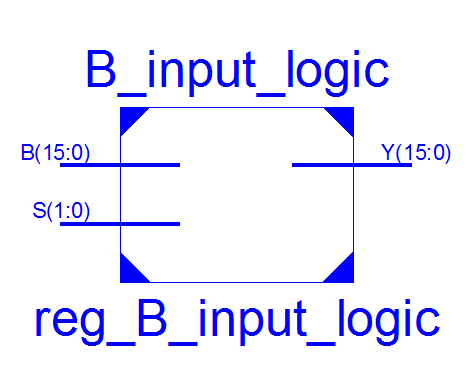
\includegraphics[width=6cm, height=8cm]{binput1.png}
\pagebreak


\subsubsection{MUX2 TO 1BIT}\label{sec:result}

\begin{lstlisting}
library IEEE;
use IEEE.STD_LOGIC_1164.ALL;


entity mux2_1bit is
    Port ( S0 : in  STD_LOGIC;
           S1 : in  STD_LOGIC;
           Cin : in  STD_LOGIC;
           Res : out  STD_LOGIC);
end mux2_1bit;

architecture Behavioral of mux2_1bit is

begin
Res <= S0 after 1ns when Cin = '1' else
			S1 after 1ns when Cin = '1' else
			'0' after 1ns;

end Behavioral;
\end{lstlisting}

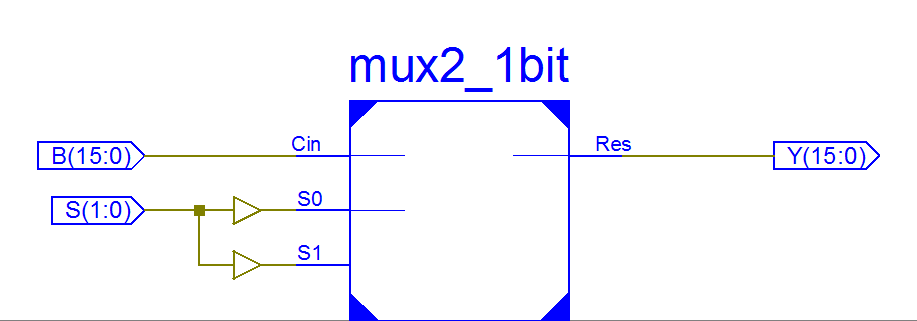
\includegraphics[width=6cm, height=8cm]{mux2to1.png}
\pagebreak



\subsubsection{RIPPLE}\label{sec:result}

\begin{lstlisting}
library IEEE;
use IEEE.STD_LOGIC_1164.ALL;
use IEEE.STD_LOGIC_ARITH.ALL;
use IEEE.STD_LOGIC_UNSIGNED.ALL;


entity ripple_adder is
    Port ( A : in  STD_LOGIC_VECTOR(15 downto 0);
           B : in  STD_LOGIC_VECTOR(15 downto 0);
           Cin : in  STD_LOGIC;
           Cout : out  STD_LOGIC;
           Gout : out  STD_LOGIC_VECTOR(15 downto 0);
           Vout : out  STD_LOGIC);
end ripple_adder;

architecture Behavioral of ripple_adder is

Component full_adder
PORT(X: in STD_LOGIC;
		Y: in STD_LOGIC;
		S: out STD_LOGIC;
		Cin: in STD_LOGIC;
		Cout: out STD_LOGIC);
End Component;

signal src_sig0, src_sig1, src_sig2, src_sig3, src_sig4,
 src_sig5, src_sig6, src_sig7, src_sig8, src_sig9, src_sig10,
 src_sig11, src_sig12, src_sig13, src_sig14, src_sig15,
 src_out: STD_LOGIC;
begin
full_adder00 : full_adder PORT MAP(X => A(0),
												Y => B(0),
												S => Gout(0),
												Cin => Cin,
												Cout =>src_sig0 );

full_adder01 : full_adder PORT MAP(X => A(1),
												Y => B(1),
												S => Gout(1),
												Cin => Cin,
												Cout =>src_sig1);
												
full_adder02 : full_adder PORT MAP(X => A(2),
												Y => B(2),
												S => Gout(2),
												Cin => Cin,
												Cout =>src_sig2);

full_adder03 : full_adder PORT MAP(X => A(3),
												Y => B(3),
												S => Gout(3),
												Cin => Cin,
												Cout =>src_sig3);

full_adder04 : full_adder PORT MAP(X => A(4),
												Y => B(4),
												S => Gout(4),
												Cin => Cin,
												Cout =>src_sig4);

full_adder05 : full_adder PORT MAP(X => A(5),
												Y => B(5),
												S => Gout(5),
												Cin => Cin,
												Cout =>src_sig5);
												
full_adder06 : full_adder PORT MAP(X => A(6),
												Y => B(6),
												S => Gout(6),
												Cin => Cin,
												Cout =>src_sig6);

full_adder07 : full_adder PORT MAP(X => A(7),
												Y => B(7),
												S => Gout(7),
												Cin => Cin,
												Cout =>src_sig7);
												
full_adder08 : full_adder PORT MAP(X => A(8),
												Y => B(8),
												S => Gout(8),
												Cin => Cin,
												Cout =>src_sig8);

full_adder09 : full_adder PORT MAP(X => A(9),
												Y => B(9),
												S => Gout(9),
												Cin => Cin,
												Cout =>src_sig9);
												
full_adder10 : full_adder PORT MAP(X => A(10),
												Y => B(10),
												S => Gout(10),
												Cin => Cin,
												Cout =>src_sig10);

full_adder11 : full_adder PORT MAP(X => A(11),
												Y => B(11),
												S => Gout(11),
												Cin => Cin,
												Cout =>src_sig11);

full_adder12 : full_adder PORT MAP(X => A(12),
												Y => B(12),
												S => Gout(12),
												Cin => Cin,
												Cout =>src_sig12);

full_adder13 : full_adder PORT MAP(X => A(13),
												Y => B(13),
												S => Gout(13),
												Cin => Cin,
												Cout =>src_sig13);
												
full_adder14 : full_adder PORT MAP(X => A(14),
												Y => B(14),
												S => Gout(14),
												Cin => Cin,
												Cout =>src_sig14);

full_adder15 : full_adder PORT MAP(X => A(15),
												Y => B(15),
												S => Gout(15),
												Cin => Cin,
												Cout =>src_sig15);



end Behavioral;
\end{lstlisting}

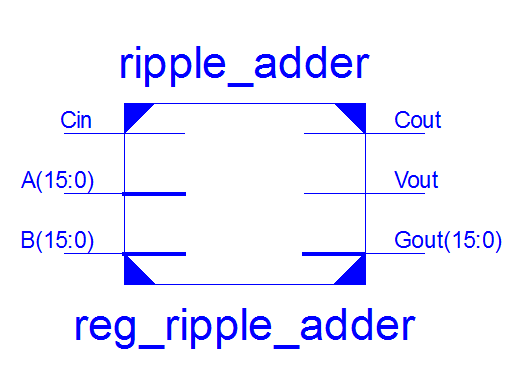
\includegraphics[width=6cm, height=8cm]{ripple.png}
\pagebreak



\subsubsection{FULL ADDER}\label{sec:result}

\begin{lstlisting}
library IEEE;
use IEEE.STD_LOGIC_1164.ALL;
use IEEE.STD_LOGIC_ARITH.ALL;
use IEEE.STD_LOGIC_UNSIGNED.ALL;


entity full_adder is
PORT(X: in STD_LOGIC;
		Y: in STD_LOGIC;
		S: out STD_LOGIC;
		Cin: in STD_LOGIC;
		Cout: out STD_LOGIC);
end full_adder;

architecture Behavioral of full_adder is

	signal S1, S2, S3: STD_LOGIC;
begin
	S1 <= (X xor Y) after 1ns;
	S2 <= (Cin and S1) after 1ns;
	S3 <= (X and Y) after 1ns;
	S <= (S1 xor Cin) after 1ns;
	Cout <= (S2 or S3) after 1ns;

end Behavioral;
\end{lstlisting}

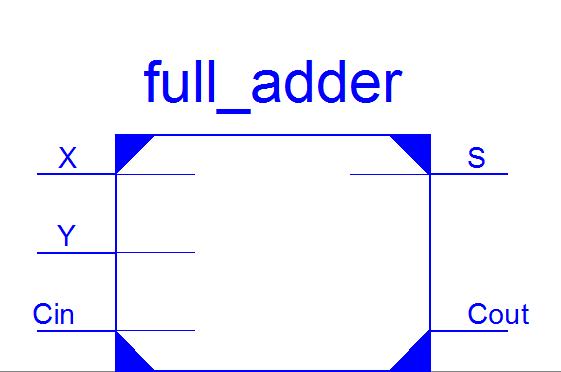
\includegraphics[width=6cm, height=8cm]{adder.png}
\pagebreak

\section{TESTBENCHES}

\subsection{DATA PATH}\label{sec:result}

\begin{lstlisting}
------------------------------------------
LIBRARY ieee;
USE ieee.std_logic_1164.ALL;
 

 
ENTITY test_datapath IS
END test_datapath;
 
ARCHITECTURE behavior OF test_datapath IS 
 
    COMPONENT datapath
    PORT(
         data_in : IN  std_logic_vector(15 downto 0);
         constant_in : IN  std_logic_vector(15 downto 0);
         D_select : IN  std_logic_vector(16 downto 0);
         D_Clk : IN  std_logic;
         D_Vout : OUT  std_logic;
         D_Cout : OUT  std_logic;
         D_Nout : OUT  std_logic;
         D_Zout : OUT  std_logic;
         address_out : OUT  std_logic_vector(15 downto 0);
         data_out : OUT  std_logic_vector(15 downto 0)
        );
    END COMPONENT;
    

   --Inputs
   signal data_in : std_logic_vector(15 downto 0) := (others => '0');
   signal constant_in : std_logic_vector(15 downto 0) := (others => '0');
   signal D_select : std_logic_vector(16 downto 0) := (others => '0');
   signal D_Clk : std_logic := '0';

 	--Outputs
   signal D_Vout : std_logic;
   signal D_Cout : std_logic;
   signal D_Nout : std_logic;
   signal D_Zout : std_logic;
   signal address_out : std_logic_vector(15 downto 0);
   signal data_out : std_logic_vector(15 downto 0);

   -- Clock period definitions
   constant D_Clk_period : time := 10 ns;
 
BEGIN
 
	-- Instantiate the Unit Under Test (UUT)
   uut: datapath PORT MAP (
          data_in => data_in,
          constant_in => constant_in,
          D_select => D_select,
          D_Clk => D_Clk,
          D_Vout => D_Vout,
          D_Cout => D_Cout,
          D_Nout => D_Nout,
          D_Zout => D_Zout,
          address_out => address_out,
          data_out => data_out
        );

   -- Clock process definitions
   D_Clk_process :process
   begin
		D_Clk <= '0';
		wait for D_Clk_period/2;
		D_Clk <= '1';
		wait for D_Clk_period/2;
   end process;
 

   -- Stimulus process
   stim_proc: process
   begin		
      data_in <= x"FFFF";
		constant_in <= x"0000";
		D_select <= "00000000100000011";
		
		wait for 20ns;
		data_in <= x"AAAA";
		D_select <= "00000000100000011";
		
		wait for 20ns;
		D_select <= "00000000100110001";
		
		wait for 20ns;
		D_select <= "01001001001000000";
		
		

      wait;
   end process;

END;
\end{lstlisting}
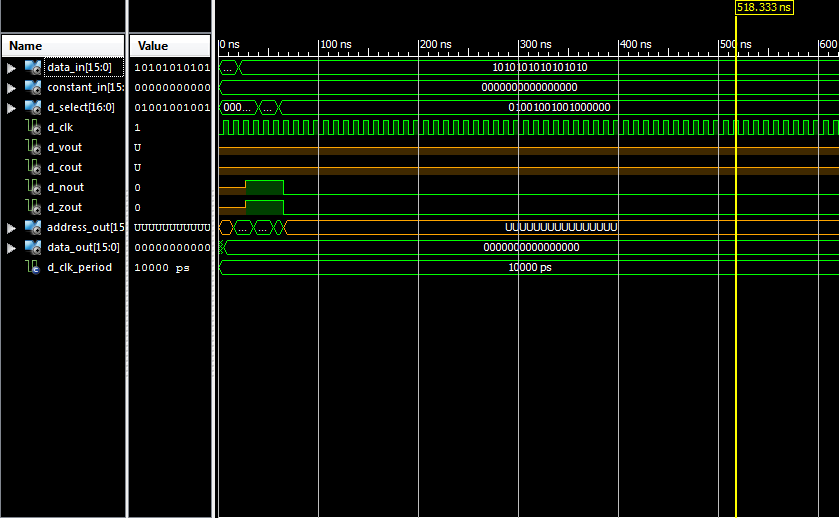
\includegraphics[width=10cm, height=5cm]{test_data.png}
\pagebreak

\subsection{REGISTER FILE}\label{sec:result}

\begin{lstlisting}

LIBRARY ieee;
USE ieee.std_logic_1164.ALL;
 

 
ENTITY test_register_file IS
END test_register_file;
 
ARCHITECTURE behavior OF test_register_file IS 
 
    -- Component Declaration for the Unit Under Test (UUT)
 
    COMPONENT register_file
    PORT(
         inA : IN  std_logic_vector(2 downto 0);
         inB : IN  std_logic_vector(2 downto 0);
         inD : IN  std_logic_vector(2 downto 0);
         Clk : IN  std_logic;
         load_in : IN  std_logic;
         data : IN  std_logic_vector(15 downto 0);
         outA : OUT  std_logic_vector(15 downto 0);
         outB : OUT  std_logic_vector(15 downto 0)
        );
    END COMPONENT;
    

   --Inputs
   signal inA : std_logic_vector(2 downto 0) := (others => '0');
   signal inB : std_logic_vector(2 downto 0) := (others => '0');
   signal inD : std_logic_vector(2 downto 0) := (others => '0');
   signal Clk : std_logic := '0';
   signal load_in : std_logic := '0';
   signal data : std_logic_vector(15 downto 0) := (others => '0');

 	--Outputs
   signal outA : std_logic_vector(15 downto 0);
   signal outB : std_logic_vector(15 downto 0);

   -- Clock period definitions
   constant Clk_period : time := 10 ns;
 
BEGIN
 
	-- Instantiate the Unit Under Test (UUT)
   uut: register_file PORT MAP (
          inA => inA,
          inB => inB,
          inD => inD,
          Clk => Clk,
          load_in => load_in,
          data => data,
          outA => outA,
          outB => outB
        );

   -- Clock process definitions
   Clk_process :process
   begin
		Clk <= '0';
		wait for Clk_period/2;
		Clk <= '1';
		wait for Clk_period/2;
   end process;
 

   -- Stimulus process
   stim_proc: process
   begin		
    load_in <= '1';
	 inD <= "000";
	 data <= x"FFFF";
	 
	 wait for 10ns;
	 inD <= "001";
	 data <= x"EEEE";
	 
	 wait for 10ns;
	 inD <= "010";
	 data <= x"DDDD";
	 
	 wait for 10ns;
	 inD <= "011";
	 data <= x"CCCC";
	 
	 wait for 10ns;
	 inD <= "100";
	 data <= x"BBBB";
	 
	 	 wait for 10ns;
	 inD <= "101";
	 data <= x"AAAA";
	 
	 wait for 10ns;
	 inD <= "110";
	 data <= x"9999";
	 
	 wait for 10ns;
	 inD <= "111";
	 data <= x"8888";
	 
	 wait for 10ns;
	 load_in <= '0';
	 inA <= "000";
	 inB <= "111";
	 
	 wait for 5ns;
	 inA <= "001";
	 inB <= "110";
	 
	 wait for 5ns;
	 inA <= "010";
	 inB <= "101";
	 
	 wait for 5ns;
	 inA <= "011";
	 inB <= "100";
	 
      wait;
   end process;

END;
\end{lstlisting}

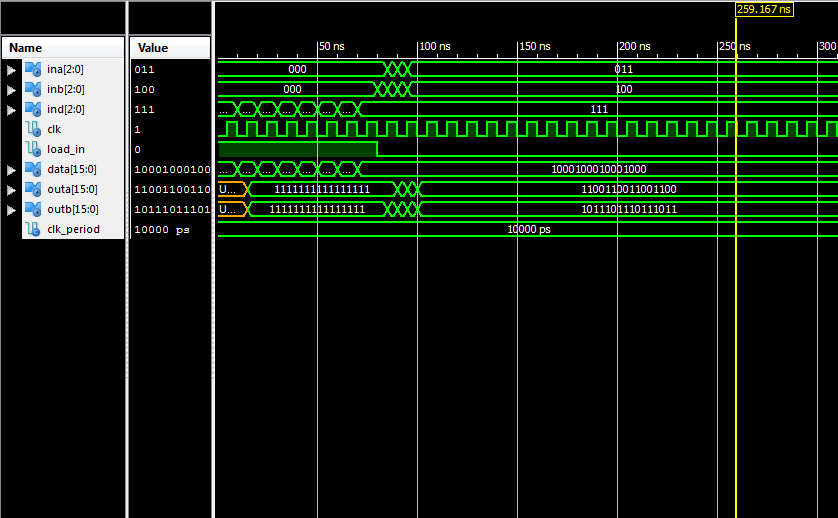
\includegraphics[width=16cm, height=8cm]{test_register_file.png}
\pagebreak

\subsubsection{REG8}\label{sec:result}

\begin{lstlisting}

LIBRARY ieee;
USE ieee.std_logic_1164.ALL;

 
ENTITY test_reg8 IS
END test_reg8;
 
ARCHITECTURE behavior OF test_reg8 IS 
 
    -- Component Declaration for the Unit Under Test (UUT)
 
    COMPONENT reg8
    PORT(
         load0 : IN  std_logic;
         load1 : IN  std_logic;
         Clk : IN  std_logic;
         D : IN  std_logic_vector(15 downto 0);
         Q : OUT  std_logic_vector(15 downto 0)
        );
    END COMPONENT;
    

   --Inputs
   signal load0 : std_logic := '0';
   signal load1 : std_logic := '0';
   signal Clk : std_logic := '0';
   signal D : std_logic_vector(15 downto 0) := (others => '0');

 	--Outputs
   signal Q : std_logic_vector(15 downto 0);

   -- Clock period definitions
   constant Clk_period : time := 10 ns;
 
BEGIN
 
	-- Instantiate the Unit Under Test (UUT)
   uut: reg8 PORT MAP (
          load0 => load0,
          load1 => load1,
          Clk => Clk,
          D => D,
          Q => Q
        );

   -- Clock process definitions
   Clk_process :process
   begin
		Clk <= '0';
		wait for Clk_period/2;
		Clk <= '1';
		wait for Clk_period/2;
   end process;
 

   -- Stimulus process
   stim_proc: process
   begin		
		D <= x"FFFF";
		load0 <= '1';
		load1 <= '1';
		
		wait for 15ns;
		D <= x"AAAA";
		load0 <= '0';
		
		wait for 10ns;
		load1 <= '0';
		
		wait for 10ns;
		load0 <= '1';
		load1 <= '1';

      wait;
   end process;

END;
\end{lstlisting}
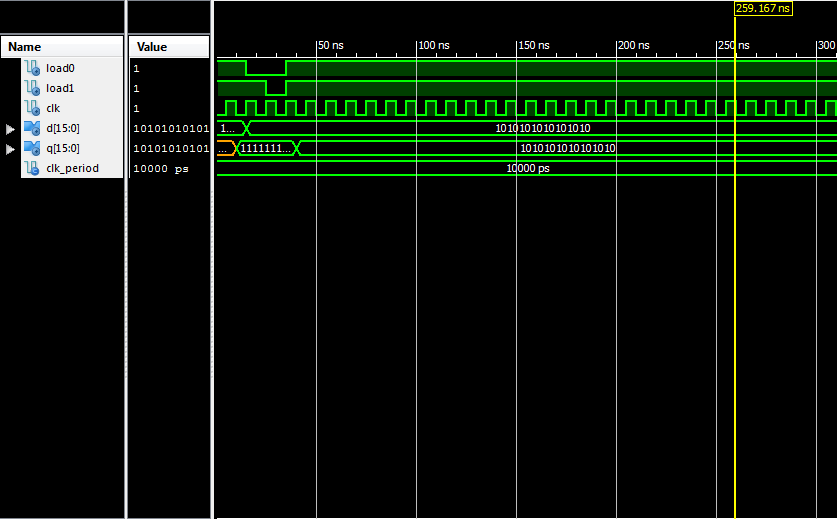
\includegraphics[width=16cm, height=8cm]{test_reg8.png}
\pagebreak
\subsubsection{DECODER}\label{sec:result}

\begin{lstlisting}

LIBRARY ieee;
USE ieee.std_logic_1164.ALL;

 
ENTITY test_decoder_3to8 IS
END test_decoder_3to8;
 
ARCHITECTURE behavior OF test_decoder_3to8 IS 
 
    -- Component Declaration for the Unit Under Test (UUT)
 
    COMPONENT decoder_3to8
    PORT(
         A0 : IN  std_logic;
         A1 : IN  std_logic;
         A2 : IN  std_logic;
         Q0 : OUT  std_logic;
         Q1 : OUT  std_logic;
         Q2 : OUT  std_logic;
         Q3 : OUT  std_logic;
         Q4 : OUT  std_logic;
         Q5 : OUT  std_logic;
         Q6 : OUT  std_logic;
         Q7 : OUT  std_logic
        );
    END COMPONENT;
    

   --Inputs
   signal A0 : std_logic := '0';
   signal A1 : std_logic := '0';
   signal A2 : std_logic := '0';

 	--Outputs
   signal Q0 : std_logic;
   signal Q1 : std_logic;
   signal Q2 : std_logic;
   signal Q3 : std_logic;
   signal Q4 : std_logic;
   signal Q5 : std_logic;
   signal Q6 : std_logic;
   signal Q7 : std_logic;
 
 
BEGIN
 
	-- Instantiate the Unit Under Test (UUT)
   uut: decoder_3to8 PORT MAP (
          A0 => A0,
          A1 => A1,
          A2 => A2,
          Q0 => Q0,
          Q1 => Q1,
          Q2 => Q2,
          Q3 => Q3,
          Q4 => Q4,
          Q5 => Q5,
          Q6 => Q6,
          Q7 => Q7
        );

 
   stim_proc: process
   begin		
     
		wait for 5ns;
		   A0 <= '0';
			A1 <= '0';
         A2 <= '0';
			
		wait for 5ns;
		   A0 <= '1';
			A1 <= '0';
         A2 <= '0';
			
		wait for 5ns;
		   A0 <= '0';
			A1 <= '1';
         A2 <= '0';
			
		wait for 5ns;
		   A0 <= '1';
			A1 <= '1';
         A2 <= '0';
			
		wait for 5ns;
		   A0 <= '0';
			A1 <= '0';
         A2 <= '1';
			
		wait for 5ns;
		   A0 <= '1';
			A1 <= '0';
         A2 <= '1';
			
		wait for 5ns;
		   A0 <= '0';
			A1 <= '1';
         A2 <= '1';
			
		wait for 5ns;
		   A0 <= '1';
			A1 <= '1';
         A2 <= '1';
		
		
      wait;
   end process;

END;
\end{lstlisting}
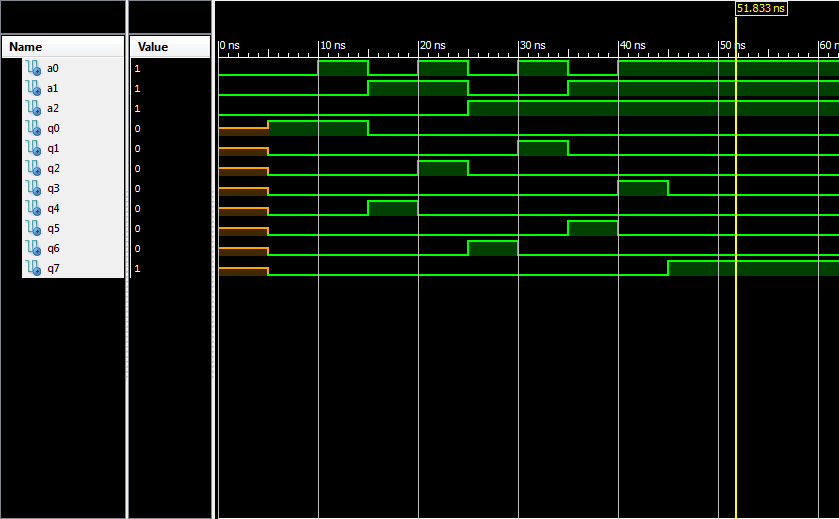
\includegraphics[width=16cm, height=8cm]{test_decoder.png}

\pagebreak

\subsubsection{MUX3 TO 16BIT}\label{sec:result}

\begin{lstlisting}

LIBRARY ieee;
USE ieee.std_logic_1164.ALL;
 

 
ENTITY test_mux3_16bit IS
END test_mux3_16bit;
 
ARCHITECTURE behavior OF test_mux3_16bit IS 
 
    -- Component Declaration for the Unit Under Test (UUT)
 
    COMPONENT mux3_16bit
    PORT(
         s : IN  std_logic;
         In0 : IN  std_logic_vector(15 downto 0);
         In1 : IN  std_logic_vector(15 downto 0);
         Z : OUT  std_logic_vector(15 downto 0)
        );
    END COMPONENT;
    

   --Inputs
   signal s : std_logic := '0';
   signal In0 : std_logic_vector(15 downto 0) := (others => '0');
   signal In1 : std_logic_vector(15 downto 0) := (others => '0');

 	--Outputs
   signal Z : std_logic_vector(15 downto 0);
   -- No clocks detected in port list. Replace <clock> below with 
   -- appropriate port name 
 
BEGIN
 
	-- Instantiate the Unit Under Test (UUT)
   uut: mux3_16bit PORT MAP (
          s => s,
          In0 => In0,
          In1 => In1,
          Z => Z
        );

   -- Stimulus process
   stim_proc: process
   begin		
          In0 <= x"FFFF";
          In1 <= x"AAAA";
			 
			 wait for 10ns;
			 s <= '1';
			 wait for 10ns;
			 s <= '0';
			 wait for 10ns;
			 s <= '1';
      wait;
   end process;

END;
\end{lstlisting}
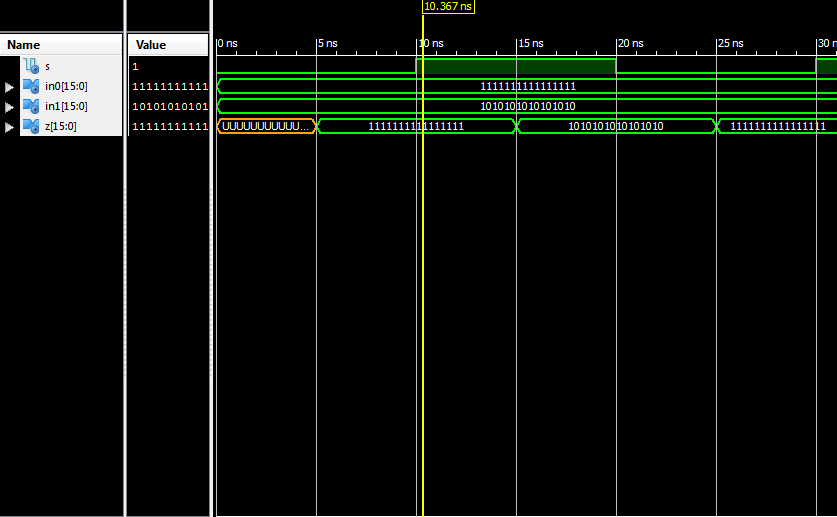
\includegraphics[width=16cm, height=8cm]{test_mux3.png}
\pagebreak

\subsubsection{MUX8 TO 16BIT}\label{sec:result}

\begin{lstlisting}

LIBRARY ieee;
USE ieee.std_logic_1164.ALL;

 
ENTITY test_mux8_16bit IS
END test_mux8_16bit;
 
ARCHITECTURE behavior OF test_mux8_16bit IS 
 
    -- Component Declaration for the Unit Under Test (UUT)
 
    COMPONENT mux8_16bit
    PORT(
         S0 : IN  std_logic;
         S1 : IN  std_logic;
         S2 : IN  std_logic;
         In0 : IN  std_logic_vector(15 downto 0);
         In1 : IN  std_logic_vector(15 downto 0);
         In2 : IN  std_logic_vector(15 downto 0);
         In3 : IN  std_logic_vector(15 downto 0);
         In4 : IN  std_logic_vector(15 downto 0);
         In5 : IN  std_logic_vector(15 downto 0);
         In6 : IN  std_logic_vector(15 downto 0);
         In7 : IN  std_logic_vector(15 downto 0);
         Z : OUT  std_logic_vector(15 downto 0)
        );
    END COMPONENT;
    

   --Inputs
   signal S0 : std_logic := '0';
   signal S1 : std_logic := '0';
   signal S2 : std_logic := '0';
   signal In0 : std_logic_vector(15 downto 0) := (others => '0');
   signal In1 : std_logic_vector(15 downto 0) := (others => '0');
   signal In2 : std_logic_vector(15 downto 0) := (others => '0');
   signal In3 : std_logic_vector(15 downto 0) := (others => '0');
   signal In4 : std_logic_vector(15 downto 0) := (others => '0');
   signal In5 : std_logic_vector(15 downto 0) := (others => '0');
   signal In6 : std_logic_vector(15 downto 0) := (others => '0');
   signal In7 : std_logic_vector(15 downto 0) := (others => '0');

 	--Outputs
   signal Z : std_logic_vector(15 downto 0);
 
BEGIN
 
	-- Instantiate the Unit Under Test (UUT)
   uut: mux8_16bit PORT MAP (
          S0 => S0,
          S1 => S1,
          S2 => S2,
          In0 => In0,
          In1 => In1,
          In2 => In2,
          In3 => In3,
          In4 => In4,
          In5 => In5,
          In6 => In6,
          In7 => In7,
          Z => Z
        );

   stim_proc: process
   begin		
		In0 <= x"FFFF";
		In1 <= x"EEEE";
		In2 <= x"DDDD";
		In3 <= x"CCCC";
		In4 <= x"BBBB";
		In5 <= x"AAAA";
		In6 <= x"9999";
		In7 <= x"8888";
		
		wait for 10ns;
		 S0 <='0';
       S1 <='0';
       S2 <='0';
		 
		wait for 10ns;
		 S0 <='1';
       S1 <='0';
       S2 <='0';
		 
		wait for 10ns;
		 S0 <='0';
       S1 <='1';
       S2 <='0';
		 
		wait for 10ns;
		 S0 <='1';
       S1 <='1';
       S2 <='0';
		 
		wait for 10ns;
		 S0 <='0';
       S1 <='0';
       S2 <='1';
		 
		wait for 10ns;
		 S0 <='1';
       S1 <='0';
       S2 <='1';
		 
		wait for 10ns;
		 S0 <='0';
       S1 <='1';
       S2 <='1';
		 
		wait for 10ns;
		 S0 <='1';
       S1 <='1';
       S2 <='1';
		
		
      wait;
   end process;

END;
\end{lstlisting}
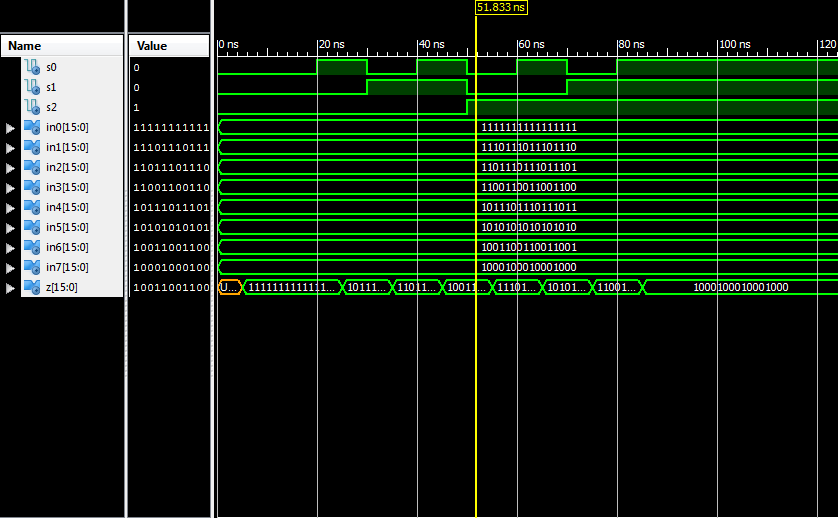
\includegraphics[width=16cm, height=8cm]{test_mux8.png}
\pagebreak


\subsection{FUNCTION UNIT}\label{sec:result}

\begin{lstlisting}

LIBRARY ieee;
USE ieee.std_logic_1164.ALL;
 

 
ENTITY test_function_unit IS
END test_function_unit;
 
ARCHITECTURE behavior OF test_function_unit IS 
 
    -- Component Declaration for the Unit Under Test (UUT)
 
    COMPONENT function_unit
    PORT(
         F_A : IN  std_logic_vector(15 downto 0);
         F_B : IN  std_logic_vector(15 downto 0);
         F_select : IN  std_logic_vector(4 downto 0);
         F_Vout : OUT  std_logic;
         F_Cout : OUT  std_logic;
         F_Nout : OUT  std_logic;
         F_Zout : OUT  std_logic;
         F_F : OUT  std_logic_vector(15 downto 0)
        );
    END COMPONENT;
    

   --Inputs
   signal F_A : std_logic_vector(15 downto 0) := (others => '0');
   signal F_B : std_logic_vector(15 downto 0) := (others => '0');
   signal F_select : std_logic_vector(4 downto 0) := (others => '0');

 	--Outputs
   signal F_Vout : std_logic;
   signal F_Cout : std_logic;
   signal F_Nout : std_logic;
   signal F_Zout : std_logic;
   signal F_F : std_logic_vector(15 downto 0);
   -- No clocks detected in port list. Replace <clock> below with 
   -- appropriate port name 
 
BEGIN
 
	-- Instantiate the Unit Under Test (UUT)
   uut: function_unit PORT MAP (
          F_A => F_A,
          F_B => F_B,
          F_select => F_select,
          F_Vout => F_Vout,
          F_Cout => F_Cout,
          F_Nout => F_Nout,
          F_Zout => F_Zout,
          F_F => F_F
        );

   -- Stimulus process
   stim_proc: process
   begin		

		F_A <= x"AAAA";
		F_B <= x"BBBB";
		
		wait for 20ns;
		F_select <= "00000";
		
		wait for 10ns;
		F_select <= "00001";
		wait for 10ns;
		F_select <= "00010";
		wait for 10ns;
		F_select <= "00011";
		wait for 20ns;
		F_select <= "00100";
		
		wait for 20ns;
		F_select <= "00101";
		wait for 20ns;
		F_select <= "00110";
		
		wait for 10ns;
		F_select <= "00111";
		wait for 10ns;
		F_select <= "01000";
		
		wait for 10ns;
		F_select <= "01001";
		wait for 10ns;
		F_select <= "01010";
		
		wait for 10ns;
		F_select <= "01011";
		wait for 10ns;
		F_select <= "01100";
		
		
		wait for 10ns;
		F_select <= "01101";
		wait for 10ns;
		F_select <= "01110";
		
		wait for 10ns;
		F_select <= "01111";
		wait for 10ns;
		F_select <= "10000";
		
		wait for 10ns;
		F_select <= "10001";
		wait for 10ns;
		F_select <= "10010";
		
		
		wait for 10ns;
		F_select <= "10011";
		wait for 10ns;
		F_select <= "10100";
		
		wait for 10ns;
		F_select <= "10101";
		wait for 10ns;
		F_select <= "10110";
		
		wait for 10ns;
		F_select <= "10111";
		wait for 10ns;
		F_select <= "11000";
		
		
		wait for 10ns;
		F_select <= "11001";
		wait for 10ns;
		F_select <= "11010";
		
		wait for 10ns;
		F_select <= "11011";
		wait for 10ns;
		F_select <= "11100";
		
		wait for 10ns;
		F_select <= "11101";
		wait for 10ns;
		F_select <= "11110";
		wait for 10ns;
		F_select <= "11111";

      wait;
   end process;

END;
\end{lstlisting}
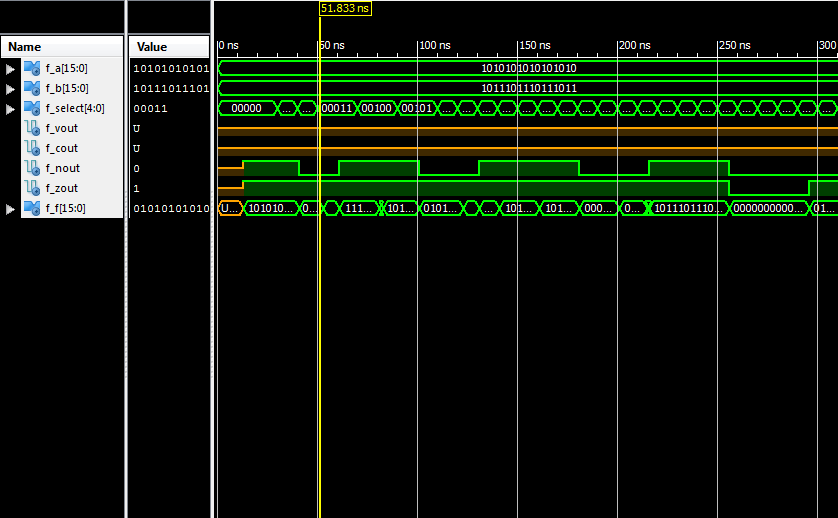
\includegraphics[width=16cm, height=8cm]{test_function_unit.png}
\pagebreak


\subsection{SHIFTER}\label{sec:result}

\begin{lstlisting}

LIBRARY ieee;
USE ieee.std_logic_1164.ALL;
 
ENTITY test_shifter IS
END test_shifter;
 
ARCHITECTURE behavior OF test_shifter IS 

    COMPONENT shifter
    PORT(
         B : IN  std_logic_vector(15 downto 0);
         S : IN  std_logic_vector(1 downto 0);
         IR : IN  std_logic;
         IL : IN  std_logic;
         H : OUT  std_logic_vector(15 downto 0)
        );
    END COMPONENT;
    

   --Inputs
   signal B : std_logic_vector(15 downto 0) := (others => '0');
   signal S : std_logic_vector(1 downto 0) := (others => '0');
   signal IR : std_logic := '0';
   signal IL : std_logic := '0';

 	--Outputs
   signal H : std_logic_vector(15 downto 0);
 
BEGIN
 
	-- Instantiate the Unit Under Test (UUT)
   uut: shifter PORT MAP (
          B => B,
          S => S,
          IR => IR,
          IL => IL,
          H => H
        );

   stim_proc: process
   begin		
    
	 wait for 10ns;
	 B <= x"FFFF";
	 S <= "00";
	 
	 wait for 15ns;
	 s <= "01";
	 
	 wait for 15ns;
	 B <= H;
	 
	 wait for 15ns;
	 B <= H;
	 S <= "10";

      wait;
   end process;

END;
\end{lstlisting}
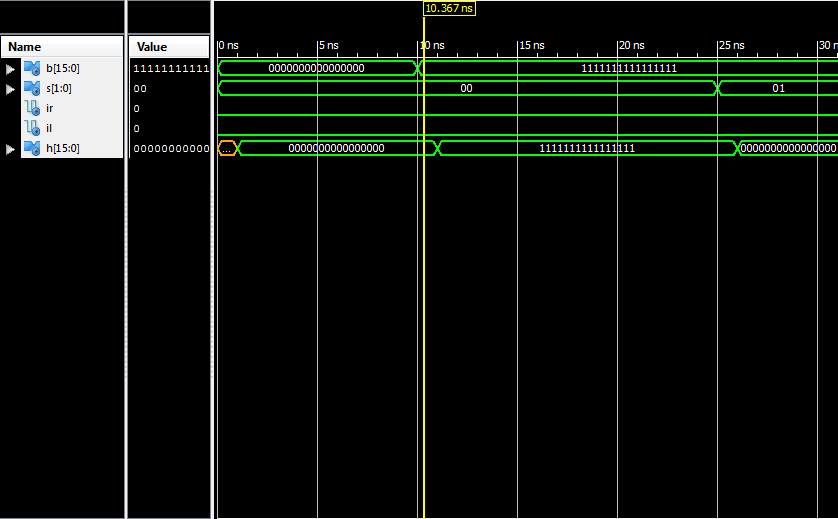
\includegraphics[width=16cm, height=8cm]{test_shifter.png}
\pagebreak


\subsubsection{MUX3 TO 1BIT}\label{sec:result}

\begin{lstlisting}

LIBRARY ieee;
USE ieee.std_logic_1164.ALL;

ENTITY test_mux3_1bit IS
END test_mux3_1bit;
 
ARCHITECTURE behavior OF test_mux3_1bit IS 
 
    -- Component Declaration for the Unit Under Test (UUT)
 
    COMPONENT mux3_1bit
    PORT(
         In0 : IN  std_logic;
         In1 : IN  std_logic;
         In2 : IN  std_logic;
         S0 : IN  std_logic;
         S1 : IN  std_logic;
         Z : OUT  std_logic
        );
    END COMPONENT;
    

   --Inputs
   signal In0 : std_logic := '0';
   signal In1 : std_logic := '0';
   signal In2 : std_logic := '0';
   signal S0 : std_logic := '0';
   signal S1 : std_logic := '0';

 	--Outputs
   signal Z : std_logic;

 
BEGIN
 
	-- Instantiate the Unit Under Test (UUT)
   uut: mux3_1bit PORT MAP (
          In0 => In0,
          In1 => In1,
          In2 => In2,
          S0 => S0,
          S1 => S1,
          Z => Z
        );

   stim_proc: process
   begin		
		wait for 10ns;
		In0 <= '0';
      In1 <= '0';
      In2 <= '0';
		
		wait for 10ns;
		In0 <= '1';
      In1 <= '0';
      In2 <= '1';
		
		wait for 5ns;
		S0 <= '0';
      S1 <= '0';
		
		wait for 5ns;
		S0 <= '0';
      S1 <= '1';
		
		wait for 5ns;
		S0 <= '1';
      S1 <= '0';
      
		wait for 5ns;
		S0 <= '1';
      S1 <= '1';
      wait;
   end process;

END;
\end{lstlisting}
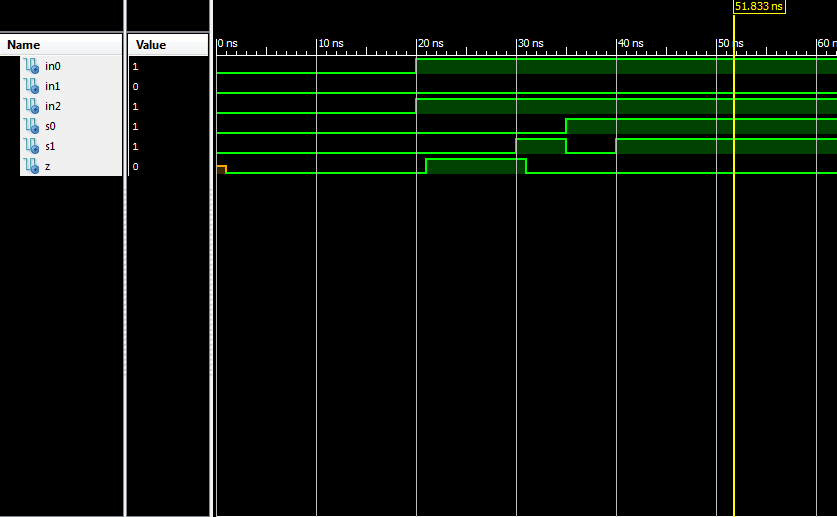
\includegraphics[width=16cm, height=8cm]{test_mux1.png}
\pagebreak




\subsection{ALU}\label{sec:result}

\begin{lstlisting}

LIBRARY ieee;
USE ieee.std_logic_1164.ALL;

ENTITY test_alu IS
END test_alu;
 
ARCHITECTURE behavior OF test_alu IS 

    COMPONENT arithmetic_logic_unit
    PORT(
         ALU_A : IN  std_logic_vector(15 downto 0);
         ALU_B : IN  std_logic_vector(15 downto 0);
         ALU_select : IN  std_logic_vector(3 downto 0);
         ALU_Cout : OUT  std_logic;
         ALU_Vout : OUT  std_logic;
         ALU_G : OUT  std_logic_vector(15 downto 0)
        );
    END COMPONENT;
    

   --Inputs
   signal ALU_A : std_logic_vector(15 downto 0) := (others => '0');
   signal ALU_B : std_logic_vector(15 downto 0) := (others => '0');
   signal ALU_select : std_logic_vector(3 downto 0) := (others => '0');

 	--Outputs
   signal ALU_Cout : std_logic;
   signal ALU_Vout : std_logic;
   signal ALU_G : std_logic_vector(15 downto 0);

BEGIN
 
	-- Instantiate the Unit Under Test (UUT)
   uut: arithmetic_logic_unit PORT MAP (
          ALU_A => ALU_A,
          ALU_B => ALU_B,
          ALU_select => ALU_select,
          ALU_Cout => ALU_Cout,
          ALU_Vout => ALU_Vout,
          ALU_G => ALU_G
        );

   stim_proc: process
   begin		
    ALU_A <= x"FFAA";
	 ALU_B <= x"000F";
	 ALU_select <= "0000";
	 
	 wait for 10ns;
	 ALU_select <= "0000";
	 
	 wait for 10ns;
	 ALU_select <= "0001";
	 
	 wait for 10ns;
	 ALU_select <= "0010";
	 
	 wait for 10ns;
	 ALU_select <= "0011";
	 
	 wait for 10ns;
	 ALU_select <= "0100";
	 
	 wait for 10ns;
	 ALU_select <= "0101";
	 
	 wait for 10ns;
	 ALU_select <= "0110";
	 
	 wait for 10ns;
	 ALU_select <= "0111";
	 
	 wait for 10ns;
	 ALU_select <= "1000";
	 
	 wait for 10ns;
	 ALU_select <= "1001";
	 
	 wait for 10ns;
	 ALU_select <= "1010";
	 
	 wait for 10ns;
	 ALU_select <= "1011";
	 
	 wait for 10ns;
	 ALU_select <= "1100";
	 
	 wait for 10ns;
	 ALU_select <= "1101";
	 
	 wait for 10ns;
	 ALU_select <= "1110";
	 
	 wait for 10ns;
	 ALU_select <= "1111";
	 
      wait;
   end process;

END;
\end{lstlisting}
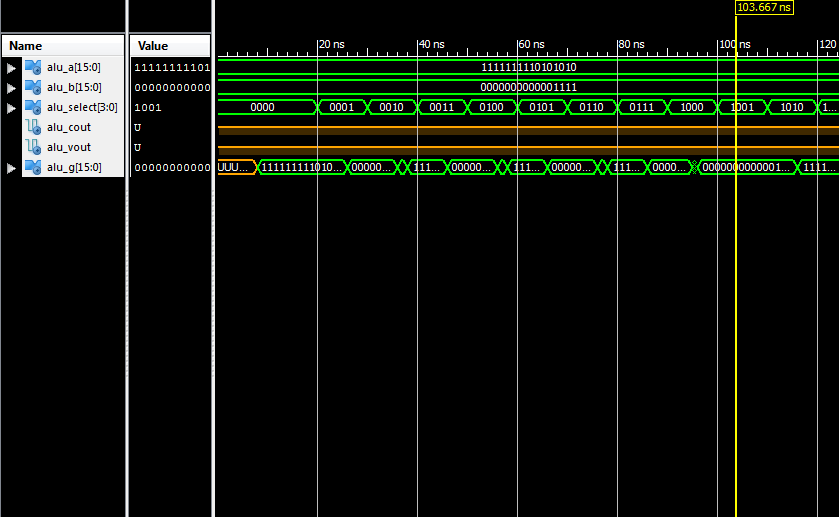
\includegraphics[width=16cm, height=8cm]{test_alu.png}
\pagebreak


\subsubsection{LOGIC}\label{sec:result}

\begin{lstlisting}

LIBRARY ieee;
USE ieee.std_logic_1164.ALL;

ENTITY test_logic IS
END test_logic;
 
ARCHITECTURE behavior OF test_logic IS 
 
    -- Component Declaration for the Unit Under Test (UUT)
 
    COMPONENT logic_circuit
    PORT(
         A : IN  std_logic_vector(15 downto 0);
         B : IN  std_logic_vector(15 downto 0);
         Cin : IN  std_logic_vector(1 downto 0);
         Cout : OUT  std_logic_vector(15 downto 0)
        );
    END COMPONENT;
    

   --Inputs
   signal A : std_logic_vector(15 downto 0) := (others => '0');
   signal B : std_logic_vector(15 downto 0) := (others => '0');
   signal Cin : std_logic_vector(1 downto 0) := (others => '0');

 	--Outputs
   signal Cout : std_logic_vector(15 downto 0);

BEGIN
 
	-- Instantiate the Unit Under Test (UUT)
   uut: logic_circuit PORT MAP (
          A => A,
          B => B,
          Cin => Cin,
          Cout => Cout
        );

   stim_proc: process
   begin		
		wait for 10ns;
		 A <= x"FFFF";
       B <= x"9999";
       Cin <= "00";
		 
		 wait for 10ns;
       Cin <= "01";
		 
		 wait for 10ns;
       Cin <= "10";
		 
		 wait for 10ns;
       Cin <= "11";
      wait;
   end process;

END;
\end{lstlisting}
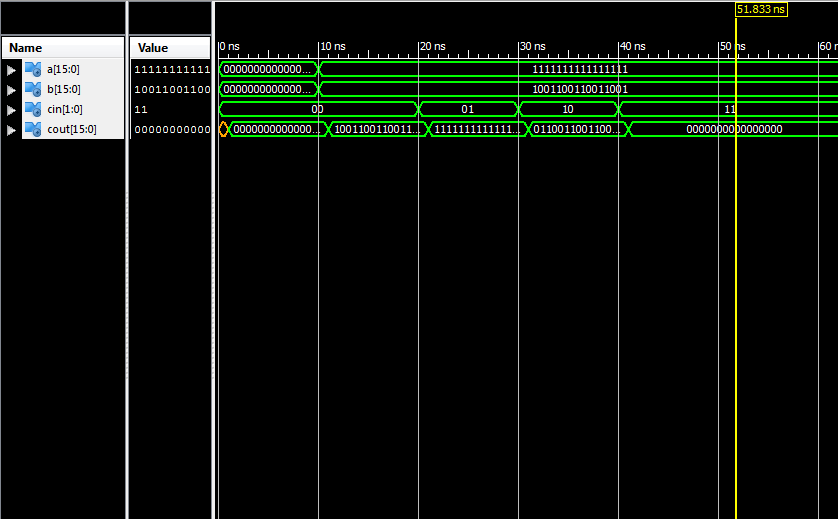
\includegraphics[width=16cm, height=8cm]{test_logic.png}
\pagebreak


\subsubsection{B LOGIC}\label{sec:result}

\begin{lstlisting}

LIBRARY ieee;
USE ieee.std_logic_1164.ALL;

ENTITY test_Blogic IS
END test_Blogic;
 
ARCHITECTURE behavior OF test_Blogic IS 

    COMPONENT B_input_logic
    PORT(
         B : IN  std_logic_vector(15 downto 0);
         S : IN  std_logic_vector(1 downto 0);
         Y : OUT  std_logic_vector(15 downto 0)
        );
    END COMPONENT;
    

   --Inputs
   signal B : std_logic_vector(15 downto 0) := (others => '0');
   signal S : std_logic_vector(1 downto 0) := (others => '0');

 	--Outputs
   signal Y : std_logic_vector(15 downto 0);

BEGIN
 
	-- Instantiate the Unit Under Test (UUT)
   uut: B_input_logic PORT MAP (
          B => B,
          S => S,
          Y => Y
        );

   stim_proc: process
   begin		
     B <=x"AAAA";
     S <= "00";

		wait for 5ns;
		S <= "00";
		wait for 5ns;
		S <= "01";
		wait for 5ns;
		S <= "10";
		wait for 5ns;
		S <= "11";
		
      wait;
   end process;

END;
\end{lstlisting}
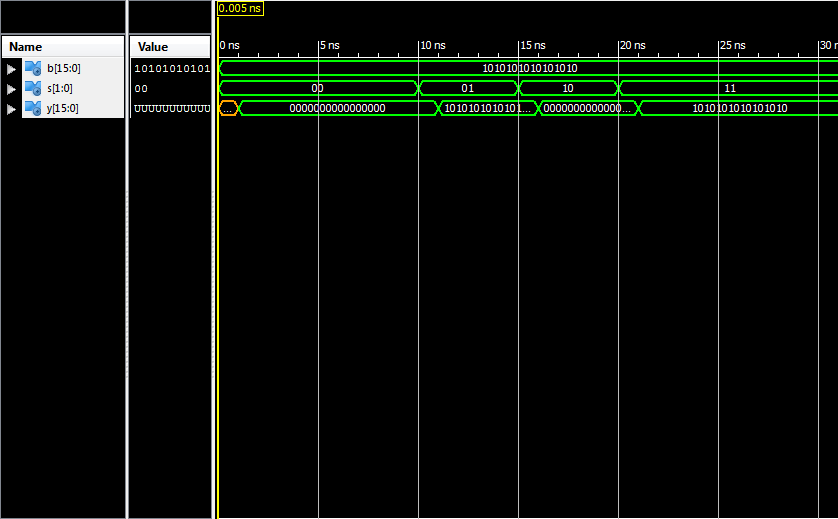
\includegraphics[width=16cm, height=8cm]{test_Blogic.png}
\pagebreak



\subsubsection{MUX2 TO 1BIT}\label{sec:result}

\begin{lstlisting}

LIBRARY ieee;
USE ieee.std_logic_1164.ALL;

ENTITY test_mux2_1bit IS
END test_mux2_1bit;
 
ARCHITECTURE behavior OF test_mux2_1bit IS 

    COMPONENT mux2_1bit
    PORT(
         S0 : IN  std_logic;
         S1 : IN  std_logic;
         Cin : IN  std_logic;
         Res : OUT  std_logic
        );
    END COMPONENT;
    
   --Inputs
   signal S0 : std_logic := '0';
   signal S1 : std_logic := '0';
   signal Cin : std_logic := '0';

 	--Outputs
   signal Res : std_logic;

BEGIN
 
	-- Instantiate the Unit Under Test (UUT)
   uut: mux2_1bit PORT MAP (
          S0 => S0,
          S1 => S1,
          Cin => Cin,
          Res => Res
        );

   stim_proc: process
   begin		
       S0 <= '1';
       S1 <=  '0';
		 
		 wait for 10ns;
		 Cin <= '1';
		 
		 wait for 10ns;
		 Cin <= '0';

      wait;
   end process;

END;
\end{lstlisting}
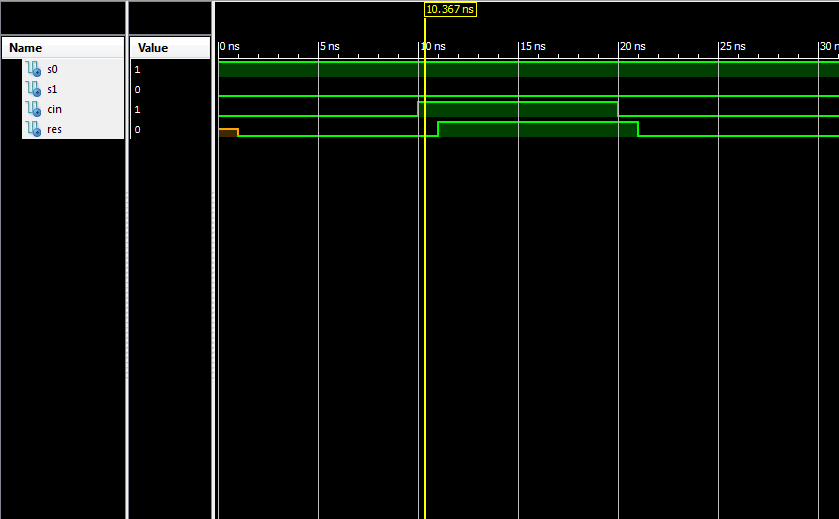
\includegraphics[width=16cm, height=8cm]{test_mux2.png}
\pagebreak


\subsubsection{RIPPLE}\label{sec:result}

\begin{lstlisting}

LIBRARY ieee;
USE ieee.std_logic_1164.ALL;

ENTITY test_ripple IS
END test_ripple;
 
ARCHITECTURE behavior OF test_ripple IS 
 
    COMPONENT ripple_adder
    PORT(
         A : IN  std_logic_vector(15 downto 0);
         B : IN  std_logic_vector(15 downto 0);
         Cin : IN  std_logic;
         Cout : OUT  std_logic;
         Gout : OUT  std_logic_vector(15 downto 0);
         Vout : OUT  std_logic
        );
    END COMPONENT;
    

   --Inputs
   signal A : std_logic_vector(15 downto 0) := (others => '0');
   signal B : std_logic_vector(15 downto 0) := (others => '0');
   signal Cin : std_logic := '0';

 	--Outputs
   signal Cout : std_logic;
   signal Gout : std_logic_vector(15 downto 0);
   signal Vout : std_logic;

BEGIN
 
	-- Instantiate the Unit Under Test (UUT)
   uut: ripple_adder PORT MAP (
          A => A,
          B => B,
          Cin => Cin,
          Cout => Cout,
          Gout => Gout,
          Vout => Vout
        );

   stim_proc: process
   begin		
	
	 A <=x"AAAA";
    B <=x"FBAA";
    Cin <= '1';
     
	  wait for 10ns;
	  A <=x"FFFF";
    B <=x"0000";
    Cin <= '1';
	  
      wait;
   end process;

END;
\end{lstlisting}
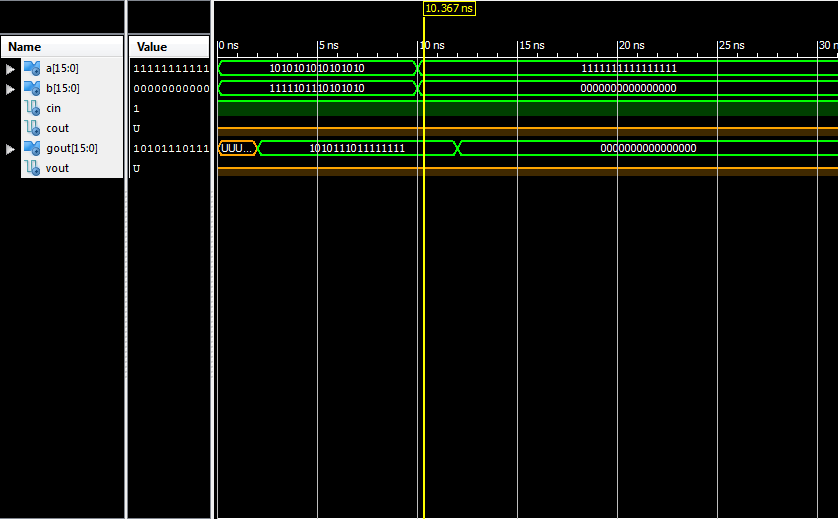
\includegraphics[width=16cm, height=8cm]{test_ripple.png}
\pagebreak


\subsubsection{FULL ADDER}\label{sec:result}

\begin{lstlisting}

LIBRARY ieee;
USE ieee.std_logic_1164.ALL;

ENTITY test_full_adder IS
END test_full_adder;
 
ARCHITECTURE behavior OF test_full_adder IS 
 
    -- Component Declaration for the Unit Under Test (UUT)
 
    COMPONENT full_adder
    PORT(
         X : IN  std_logic;
         Y : IN  std_logic;
         S : OUT  std_logic;
         Cin : IN  std_logic;
         Cout : OUT  std_logic
        );
    END COMPONENT;
    

   --Inputs
   signal X : std_logic := '0';
   signal Y : std_logic := '0';
   signal Cin : std_logic := '0';

 	--Outputs
   signal S : std_logic;
   signal Cout : std_logic;

BEGIN
 
	-- Instantiate the Unit Under Test (UUT)
   uut: full_adder PORT MAP (
          X => X,
          Y => Y,
          S => S,
          Cin => Cin,
          Cout => Cout
        );

   stim_proc: process
   begin		
	
		wait for 10ns;
		 X <= '0';
       Y <= '0';
      
		wait for 10ns;
		 X <= '0';
       Y <= '1';

		wait for 10ns;
		 X <= '1';
       Y <= '0';
      
		wait for 10ns;
		 X <= '1';
       Y <= '1';
		 
		wait for 10ns;
		 Cin <= '1';
  

      wait;
   end process;

END;
\end{lstlisting}
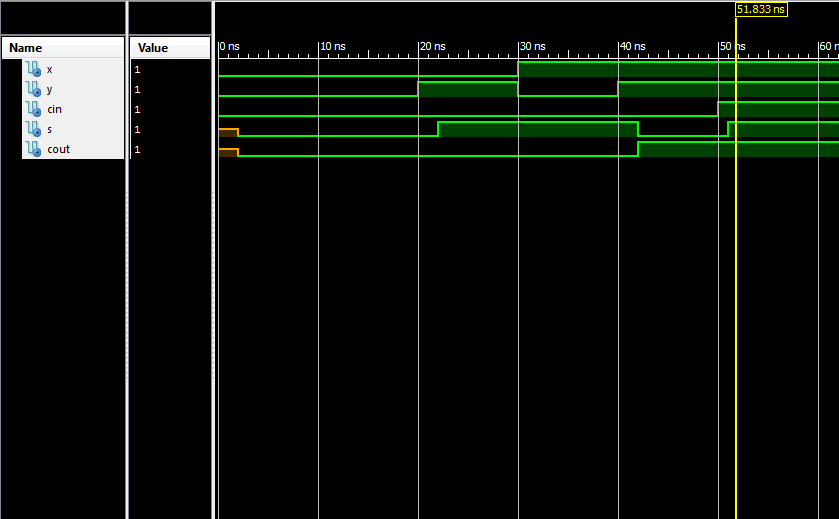
\includegraphics[width=16cm, height=8cm]{test_full.png}
\pagebreak
	
\end{document}